\chapter{Grundlagen}

\section{\acrfull{mqtt}}
\acrshort{mqtt} ist ein Protokoll, welches zur digitalen Datenübertragung in ethernet-basierten Systemen dient. Es benötigt nur wenig Bandbreite und Ressourcen und verwendet eine 
Publish/Subscribe - Architektur. Das bedeutet, dass Nachrichten sogenannter Topics von Publishern bereitgestellt und von Subscribern empfangen werden. Der Datenverkehr wird über einen 
zentralen Broker verwaltet. Um die Publish Subscribe Architektur zu verstehen ist es hilfreich die Analogie zum Fernsehen zu bilden. Dabei sendet ein TV-Sender sein Programm an einen bestimmten Kanal.
Auf diesen Kanal können nun beliebig viele Fernseher (Subscriber) zugreifen. Auch wenn keine aktive Verbindung zwischen Sender und Empfänger aufgebaut wird, erhalten beliebig viele Empfänger die benötigten Daten.
In \autoref{pic:mqttbroker} ist zu erkennen, wie die Daten nicht zwischen Publisher und Subscriber direkt, sondern über den zentralen Broker versendet werden. (Vgl. \cite{mqtt})

\begin{figure}[h]
    \begin{center}
        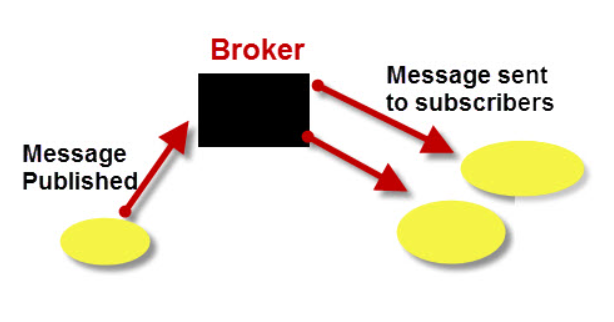
\includegraphics[width=8cm]{mqttbroker.png}
        \caption{\acrshort{mqtt}-Datenübertragung über den Broker}
        \label{pic:mqttbroker}
    \end{center}
\end{figure}